\chapter{Introduction}
\label{chap:intro}

%%%%%%%%%%%%%%%%%%%%%%%%%%%%%%%%%%%%%%%%%%%%%%%%%
%%%%%%%%%%%%%%%%%%%%%%%%%%%%%%%%%%%%%%%%%%%%%%%%%
%%%%%%%%%%%%%%%%%%%%%%%%%%%%%%%%%%%%%%%%%%%%%%%%%
\section{Exoplanet Observations}
\subsection{Detection Methods}
\subsubsection{Radial Velocity}
\label{sec:RV}
A periodic wobble will be observed in the lightcurve of a star with an orbiting planet, due to their coupled motion around the common centre of mass. 
From the conservation of energy and angular momentum, a star's wobble (or radial velocity) due to a planetary companion can be calculated according to \citep{Beauge2007}:
\begin{equation}
V_r = K \cdot [\cos(\nu + \omega) + e\cdot \cos(\omega) + \gamma]
\label{eq:RV}
\end{equation}
where $K$ is the semi-amplitude:
\begin{equation}
K = \frac{m_p \sin(i)}{m_* + m_p} \frac{2\pi a}{P\sqrt{1-e^2}}
\label{eq:K}
\end{equation}
$a$ is the semi-major axis of the planet, $P$ is the orbital period, $m_p$ is the planet mass, $m_*$ is the stellar mass, $i$ is the inclination, $e$ is the eccentricity, $\nu$ is the true anomaly, $\omega$ is the argument of periastron, and $\gamma$ is the stellar drift in velocity.
Since the probability of detecting a planet is related to $K$, radial velocity preferentially detects massive planets on short orbits. 

From Equations~\ref{eq:RV} and \ref{eq:K}, one can extract many orbital parameters of the planet including $e$, $a$, and $m_p\sin(i)$.
However, successful extraction of these orbital parameters requires accurate and precise knowledge of the stellar mass, which is often difficult to obtain \citep[e.g.][]{Brown2011}.
Furthermore, only a lower limit estimate on planet mass can be calculated unless the inclination relative to Earth's line of sight is known. 
In addition, the radius of the planet cannot be determined from the radial velocity method, precluding information about size and density.

When multiple planets orbit a star, the radial velocity signal becomes more complicated.
Assuming that the planets are well-separated such that their mutual gravitational interactions are weak, the radial velocity of the star can be approximated as the sum of planetary Keplerian orbits:
\begin{equation}
V_r = \gamma + \sum_{i=1}^{n_p} K_i \cdot [\cos(\nu_i + \omega_i) + e_i\cdot \cos(\omega_i)]
\label{eq:RVsum}
\end{equation}
where $n_p$ is the number of planets in the system. 
If however the planet-planet gravitational interactions are strong, Equation~\ref{eq:RVsum} is invalid and must be replaced with a more careful numerical treatment. 
Chapter~\ref{chap:HD155358} presents such a detailed numerical treatment, which builds off the work of  \citet{Robertson2012} who used Equation~\ref{eq:RVsum} to extract the orbital parameters of the HD155358 system, which hosts two Jovian-sized planets near mean motion resonance. 

\subsubsection{Transit Method}
\label{sec:transit}
When a planet passes (or transits) in front of its host star, a portion of the star's emitted flux $F$ will be blocked. 
The fraction of blocked flux is proportional to the relative areas of the star and planet:
\begin{equation}
\frac{\Delta F}{F} \propto \left(\frac{r_p}{r_*}\right)^2
\label{eq:F}
\end{equation}
where $r_p$ and $r_*$ are the planet and stellar radii, respectively. 
In addition, the probability of a transiting planet $P_t$ is inversely proportional to its semi-major axis:
\begin{equation}
P_t = \frac{r_*}{a}
\label{eq:tp}
\end{equation}
Thus, from Equations~\ref{eq:F} and \ref{eq:tp} we see that large, short-period planets are preferentially detected by the transit method.

The first transiting planet was detected by \citet{Henry1999} and independently by \citet{Charbonneau2000}.
Since then the transit method has become the most successful detection technique, with over 2,700 confirmed planets to date \citep{Akeson2013}. 
Most of these discoveries have come from the \textit{Kepler Space Telescope} (hereafter \kep).
For reference, the next most successful detection technique is the radial velocity method (Section~\ref{sec:RV}) with over 600 confirmed planets to date \citep{Akeson2013}.

From the transit method one can determine the period and radius of the planet. 
In addition, the atmospheric properties of exoplanets can also be probed \citep{Kreidberg2014, Tsiaras2016, Stevenson2016}.
In total, the transit method is able to provide essential information about the composition, formation and habitability of a planet. 
However, the transit method has several weaknesses. 
For example, most orbital parameters required for dynamical studies, like eccentricity and mass, cannot be determined for individual systems via the transit method alone\footnote{When neighbouring planets exhibit Transit Timing Variations, information can be collected about eccentricity and mass \citep{Holman2005}.}.
In addition, false positives from eclipsing binaries and background targets are a significant source of contamination \citep{Fressin2013}, and confirmation via a different method is often required. 
Smaller planets and/or planets belonging to multi-planet systems are much less likely to be false positives than large, single planets \citep{Fressin2013, Lissauer2011}.

\subsection{Statistics of Kepler Planets}
\label{sec:stats}
%I'm assuming that since this section is meant to motivate my work, I should focus on the research leading up to mine, not the research that has happened since.
The \kep mission is the most successful planet-finding mission to date, providing scientists for the first time a population of planets orbiting other stars. 
Due to the selection bias of the transit method (see Section~\ref{sec:transit}), most of these planets have periods of less than 50 days and are larger than Earth. 
However, sufficient detection across the full range of Earth-to-Jupiter sized planets has enabled scientists to calculate the occurrence of planets around stars in our galaxy. 

Two seminal works analyzing the \kep population are \citet{Fressin2013} and \citet{Petigura2013}.
\citet{Fressin2013} found that the global false positive rate of the \kep data is roughly $10\%$, the radius distribution peaks at mini-Neptune sized planets ($2<r_p/r_{\oplus}<2.8$, $r_{\oplus}$ is the radius of Earth), and the occurrence of Neptune and Jupiter sized planets is significantly lower than the occurrence of $r_p/r_{\oplus}<2.8$ sized planets.
Using a carefully vetted data sample, \citet{Petigura2013} found a similar result as \citet{Fressin2013}, i.e. that the radius distribution peaks at mini-Neptune and the occurrence of Neptune and Jupiter sized planets is much lower.

A calculation of planet occurrence is usually performed by binning the planets in $r$--$P$ space (where $r$ is planet radius and $P$ is planet period), and calculating planet occurrence for each bin. 
The occurrence $f(P_i, r_j)$ of planets in bin $(i,j)$ for a population of planets is:
\begin{equation}
f(P_i, r_j) = \frac{1}{N_*} \sum_k^{n_p(i,j)} \left(\frac{a_k}{r_{*,k}} \frac{1}{\epsilon(i,j)} \right)
\label{eq:occurence}
\end{equation}
where $N_*$ is the total number of stars surveyed in the sample, $n_p(i, j)$ are the number of planets falling into bin $(i, j)$, $\frac{a_k}{r_{*,k}}$ is the geometric correction factor to account for missed non-transiting planets (inverse of Equation~\ref{eq:tp}) and $\epsilon(i,j)$ is the detection completeness of bin $(i, j)$ to account for missed transiting planets due to low signal-to-noise.

Of the ingredients that go into Equation~\ref{eq:occurence} the most difficult to accurately measure is the detection completeness. 
Unlike \citet{Fressin2013} who used Combined Differential Photometric Precision (CDPP) values to calculate the detection completeness of known planets, \citet{Petigura2013} instead performed an injection and recovery of simulated light curves. 
Although the injection and recovery technique is certainly a more accurate way to calculate the detection completeness, \citet{Fressin2013} found that CDPP estimates were robust and could lead to accurate predictions. 

One critical aspect of planet occurrence that \citet{Fressin2013} and \citet{Petigura2013} failed to incorporate into their calculations was the large error bars present in the \kep data.
The mean planetary radius error in the \citep{Ramirez2014} \kep dataset is $30\%$, meaning that, within 3 standard deviations a super-Earth sized planet could actually be Neptune or Earth-sized. 
These errors primarily stem from the fact that the radii of \kep stars are not well known \citep{Brown2011}, also with a mean radius error of $30\%$.
With such large error bars present in the \kep data, ignoring them can affect the resulting radius and planet occurrence distributions.
Chapter~\ref{chap:Stats} performs a planet occurrence calculation similar to \citet{Fressin2013} and \citet{Petigura2013} whilst incorporating these large errors into the analysis. 

%%%%%%%%%%%%%%%%%%%%%%%%%%%%%%%%%%%%%%%%%%%%%%%%%
%%%%%%%%%%%%%%%%%%%%%%%%%%%%%%%%%%%%%%%%%%%%%%%%%
%%%%%%%%%%%%%%%%%%%%%%%%%%%%%%%%%%%%%%%%%%%%%%%%%
\section{Planet Formation}
\label{sec:PF}
\subsection{Minimum Mass Solar Nebula and Snowline}
The initial conditions of the Solar System are still largely unknown.
\citet{Hayashi1981} and \citet{Weidenschilling1977} provided the first benchmarks for the initial mass of the Solar System by assuming a rocky core for all planets and calculating the initial surface density distribution $\Sigma$ as a function of distance $d$ required to produce the masses of the planets:
\begin{equation}
\Sigma(d) = \Sigma_0\left(\frac{d}{1 \textrm{AU}} \right)^{-3/2}
\end{equation}
where $\Sigma_0 = 1700 \textrm{g/cm}^{2}$. 
This initial surface density distribution is known as the Minimum Mass Solar Nebula (MMSN), and is a benchmark against which most planet formation studies are compared to.

%berta, charbonneau 2012

A second critical property of circumstellar disks is the location of the snowline. 
In standard formation theory the snowline marks the boundary where water ice begins to form, providing the additional solid material required to make large cores and form Jovian planets.
\citet{Hayashi1981} provided a benchmark temperature profile $T(d)$ for the Solar System:
\begin{equation}
T(d) = T_0 \left(\frac{d}{1 \textrm{AU}} \right)^{-1/2}
\end{equation}
where $T_0 = 280$K. 
In this model, the distance at which the temperature drops to below freezing is $\sim 2.7$ AU. 
More recent models of the snowline \citep{Sasselov2000} include detailed radiative transfer physics and heating via accretion, and show that the primordial snow line in our Solar System could have been as close as 1 AU.

Until recently, scientists have lacked the tools to observationally test theories of early solar system formation.  
Telescopes like the Atacama Large Millimeter/submillimeter Array (ALMA) have begun providing observations of circumstellar disks around young stellar objects like HL Tau \citep{ALMA2015}.
In total, about 80 circumstellar and debris disks have been observed to date \citep[e.g.][]{Schneider2014,Choquet2016}, revealing unexpected features like strong debris disk asymmetries \citep{Hines2007}, concentric rings sculpted by possible Jovian-sized planets \citep{Tamayo2015} and highly eccentric/unbound trajectories in debris disks that are difficult to reconcile with standard formation theories \citep{Boccaletti2015}.

\subsection{Planetesimal Formation}
Before planets can form there must be an abundance of kilometre-sized planetesimals.
There are currently two leading models for forming such kilometre-sized planetesimals -- coagulation (a.k.a. core-accretion) and gravitational instability. 
In the coagulation model, pairwise collisions between sticky dust particles lead to steady growth up to meter-sized and beyond \citep{Weidenschilling1977b, Armitage2010}.
However, mean collision velocities are strongly coupled to size and destructive collisions tend to occur between meter-sized objects, hindering further planetesimal growth \citep{Weidenschilling1977b, Blum2008}. 
In addition, meter-sized objects embedded in a protoplanetary disk will strongly couple to the gas and typically drift into the central star on a timescale of $10^3$ years \citep{Weidenschilling1977b}.
Thus, a mechanism is required to quickly grow particles beyond a meter in size to avoid destruction. 
Solutions to this "meter-barrier problem" have been proposed, however no clear consensus has yet emerged.  
For example, \citet[e.g.][]{Boley2014} suggested that as meter-sized bodies drift closer to the central their they will become partially molten, increasing their stickiness and promoting further collisional growth. 

In the gravitational instability model, as the solar nebula cools dust particles settle in the mid plane, becoming vulnerable to collapse \citep{Goldreich1973}.
These dust particles clump and eventually become gravitationally unstable, forming $\sim$100m sized particles \citep{Goldreich1973}. 
This process then repeats, each time forming larger and larger planetesimals via gravitational instability.
This model is attractive since it bypasses the scales most vulnerable to destructive collisions (i.e. the meter-barrier problem), and can form large planetesimals in $\sim 10^3$ years \citep{Goldreich1973, Armitage2007}.
However, in practice it is very difficult to collect dust particles in densities high enough for gravitational instability, and especially so in turbulent disks \citep{Armitage2007}.
 
The formation mechanism of planetesimals is still unclear, however, \textit{some} mechanism must exist since planetesimals are ubiquitous. 

\subsection{Formation of Protoplanets}
The formation of protoplanets occurs shortly after the formation of large, kilometre-sized planetesimals.
In a pioneering study, \citet{Greenberg1978} found that in the early stages of planet formation larger planetesimals grow more rapidly than smaller ones, resulting in the runaway growth of the largest planetesimal. 
As a result, $1$--$10$ km sized planetesimals at $1$AU can grow into $10^{22}$ -- $10^{24}$ kg protoplanets in $10^5$--$10^6$ years \citep{Wetherill1989}.
This runaway process stems from the fact that $1$--$10$ km sized planetesimals are large enough to gravitationally focus each other yet are still dynamically cool via damping from surrounding gas, resulting in a maximum collision cross section \citep{Armitage2010}.
Since proplanetary growth rates are related to orbital frequency, more distant regions will have slower growth timescales.

Eventually this runaway growth transitions into a slower, oligarchic growth. 
As protoplanets grow surrounding planetesimals are dynamically excited via gravitational stirring, decreasing the collision cross section and slowing the rate of protoplanetary growth \citep{Kokubo1998}.
By the end of oligarchic growth protoplanets have consumed most of the surrounding material and have reached their isolation masses \citep{Schlichting2014}.
Beyond the snowline the isolation mass is roughly the mass of Neptune, however inside the snowline it is a fraction of an Earth mass \citep{Schlichting2014}.
Since numerous \kep planets larger than Earth reside inside the snowline of their host star, this suggests that either i) giant impacts between protoplanets, ii) inward drift of additional material, or iii) migration must have taken place \citep{Schlichting2014}.  

%%%%%%%%%%%%%%%%%%%%%%%%%%%%%%%%%%%%%%%%%%%%%%%%%
%%%%%%%%%%%%%%%%%%%%%%%%%%%%%%%%%%%%%%%%%%%%%%%%%
%%%%%%%%%%%%%%%%%%%%%%%%%%%%%%%%%%%%%%%%%%%%%%%%%
\section{Planetary Dynamics}
\subsection{Mean Motion Resonance}
\label{sec:MMR}
Mean motion resonance (MMR) occurs when the orbital period of one planet is an integer ratio of another. 
Like other types of resonances occuring in nature, MMR results in the amplitude growth of various quantities characterizing the system like eccentricity, semi-major axis and the longitude of pericentre \citep{SSD1999}. 
As a result, the presence of MMR can strongly affect the formation, evolution and longterm stability of planetary systems in a diversity of ways.
For example, Kirkwood gaps are unstable regions in the asteroid belt carved by MMRs with Jupiter, while Pluto and Neptune are protected from going unstable due to a 3:2 MMR. 

For every $p:q$ MMR (where $p$ and $q$ are integers) there are two important resonant angles:
\begin{align}
\begin{split}
\phi_1 &= p\lambda_1 - q\lambda_2 + \varpi_1 \\
\phi_2 &= p\lambda_1 - q\lambda_2 + \varpi_2 
\label{eq:MMR}
\end{split}
\end{align}
where $\lambda$ is the mean longitude and $\varpi$ is the longitude of periapse. 
For planets to be in MMR, the time variation of one or both resonant arguments must be zero.
As a result, MMRs can be modelled in terms of a pendulum oscillating about a stable, fixed point. 
After some algebra it can be shown that a MMR can be modelled as \citep{SSD1999}:
\begin{equation}
\ddot{\phi} = -\omega_0^2 \sin\phi
\label{eq:pendulum}
\end{equation}
where $\omega_0$ is the amplitude of libration and is dependent upon the orbital parameters of the system (mass, eccentricity, semi-major axis).

The pendulum model facilitates an understanding about certain properties of MMR. 
For energies larger than a critical energy, $E_{crit}$, the pendulum will circulate over all possible values of $\phi$, while for energies smaller than $E_{crit}$ the pendulum will be in MMR and librate about $\phi = 0$.
The critical energy, $E_{crit}$, defines motion on the separatrix, which separates the circulation and libration regimes. 
In context of a pendulum, this would correspond to the pendulum suspended vertically in the air with an infinite period of libration. 

The strength of a given MMR is related to its width, which in turn is related to the order of the resonance ($= p - q$) and the magnitude of $p$ and $q$ \citep{SSD1999}. 
More fundamentally, the strength of a MMR is related to the mass, eccentricity and mean motions of the planets involved \citep{SSD1999}.
Stronger MMRs are associated with lower values of $p$, $q$ and $p-q$, making the 2:1 and 3:2 MMRs the most probable resonant locations in nature. 
Figure~\ref{fig:KepMMR} shows the distribution of period ratios for planets discovered by \kep, along with the locations of first and second order MMRs. 
As can be seen, statistical excesses of planets exist wide of the 3:2 MMR and 2:1 MMR \citep{Lissauer2011,Fabrycky2014,Steffen2015}, and it is believed that these planets were transported away from MMR  via dissipative mechanisms.
The most popular of these dissipative mechanisms are tidal \citep{LithwickWu2012, Batygin2013, Delisle2014}, protoplanetary \citep{Rein2012b, Baruteau2013, Goldreich2014}, and planetesimal \citep{Moore2013, Chatterjee2015}.
The formation implications for each mechanism are different, and no clear consensus has yet emerged.
Chapter~\ref{chap:Tides} critically examines the role of tidal forces in transporting \kep planets from exact MMR to their observed locations, using analytical and numerical means. 

\begin{figure}
\centering
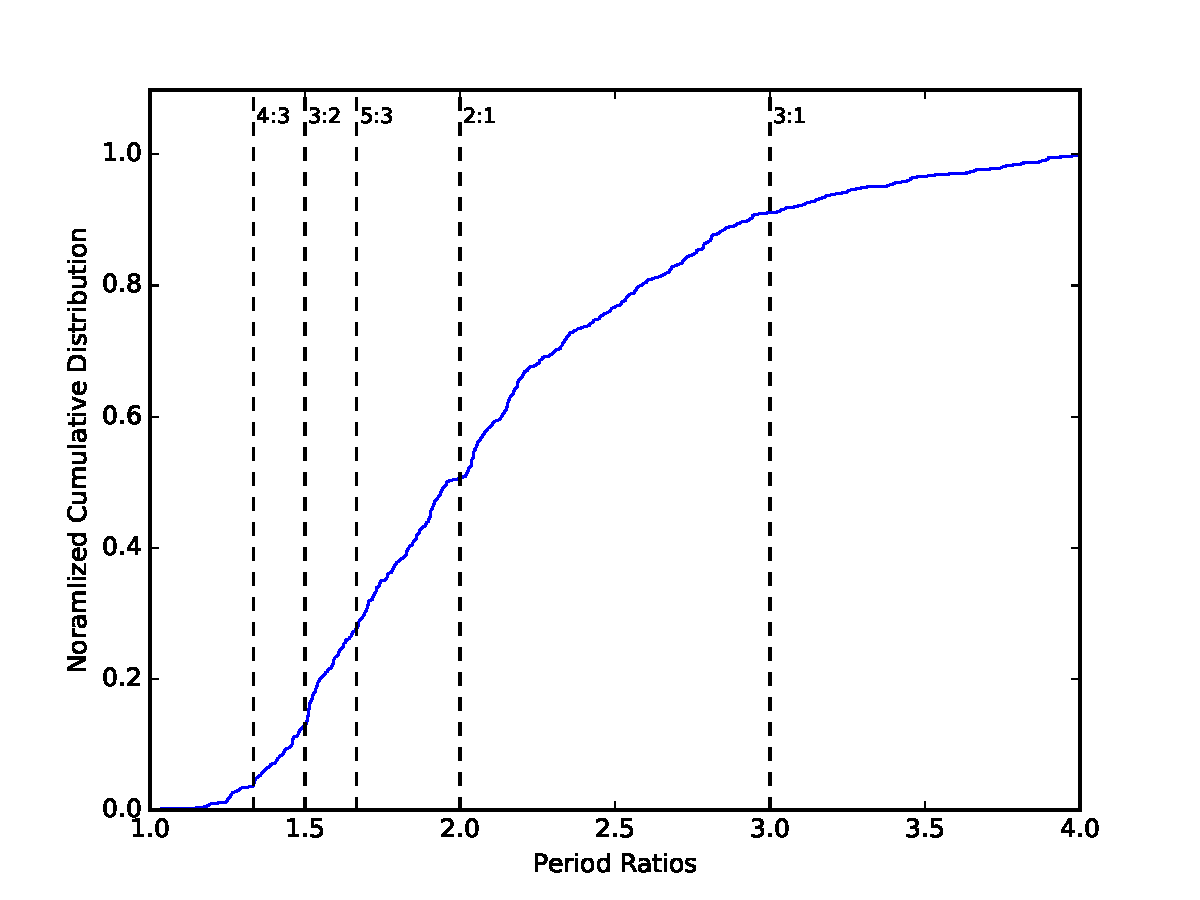
\includegraphics[width=1.00\textwidth]{intro/PeriodRatios}
\caption{
Cumulative distribution of period ratios of neighbouring planets in all known multi-planet systems.
 First and second-order mean motion resonances are displayed as dotted lines, and labelled at the top of the figure. 
 Data from \citet{Akeson2013}.}
\label{fig:KepMMR}
\end{figure}

\subsection{Migration}
\label{sec:migration}
Planetary migration is believed to be the most effective way of trapping planets in MMR \citep[e.g.][]{Lee2002}, making it a very important process for planet formation.  
Throughout this thesis (Chapters~\ref{chap:Tides}, \ref{chap:Hermes} and \ref{chap:HD155358}) migration physics is utilized, and presented here are the two primary ways that planets can migrate.

\subsubsection{Planetesimal-Driven Migration}
Planetesimals passing through the Hill sphere of a planet will exchange angular momentum via gravity \citep{Ida2000, Kirsh2009}.
If there is an asymmetry to the mass of planetesimals interacting with the planet on its near and far sides, a net force will migrate the planet. 
However, to guarantee a net migration planetesimal orbits must decouple from the planet. 
A massive enough planet (e.g. Jupiter) will directly eject and decouple planetesimals from the system, however if the planet is smaller (e.g. Neptune) planetesimals must decouple by interacting with a neighbouring planet. 
In addition, for sustained migration the planet must constantly encounter fresh, dynamically cold planetesimals \citep{Gomes2004}.  

Since protoplanetary growth is proportional to orbital frequency \citep[e.g.][]{Rafikov2003}, planetesimal disks are most likely to exist in the outer reaches of planetary systems where fewer orbital cycles have occurred. 
In the Solar System, the primordial Kuiper belt is believed to have once been such a planetesimal disk, causing Neptune to migrate outwards into the Kuiper belt and shepherd planetesimals inwards to Jupiter, which subsequently ejected them from the Solar System \citep{Fernandez1984}.
This idea is well supported by observations of the outer Solar System, which show that Pluto, along with a host of smaller bodies, orbit in stable 3:2 MMRs with Neptune \citep{Malhotra1993, Malhotra1995}.

\subsubsection{Gas-Driven migration}
Since the discovery of the first hot Jupiter \citep{Mayor1995}, gas-driven migration is believed to play an important role in shaping exoplanetary systems \citep{Lin1996}.
Whenever a fully-formed planet is embedded in a protoplanetary disk, angular momentum can be exchanged via disk-planet torques \citep{Goldreich1980}.
The result of this exchange is planetary migration, and this scenario is believed to be common to all young planetary systems. 
Gas-driven migration comes in two main flavours -- Type I and Type II. 

Type I migration occurs when low-mass planets are fully embedded in a protoplanetary disk and do not significantly perturb the disk structure \citep{Armitage2010}. 
At particular resonant locations, known as Linblad resonances, density waves are excited due to gravitational interactions between the planet and disk \citep{Goldreich1979}. 
These density waves exchange angular momentum with the planet, and migration occurs when the inner and outer disk interact asymmetrically with the planet \citep{Goldreich1979}.
In general, the direction of Type-I migration tends to be inwards towards the central star \citep{Ward1997}.

Type II migration occurs when high-mass Jovian planets significantly modify the structure of the surrounding protoplanetary disk, opening up a gap. 
This gap locks the planet in place, coupling the migration of the planet to the evolution of the disk \citep{Lin1986}.
The viscous evolution of the disk causes the planet to slowly migrate inwards, at speeds typically one or two orders of magnitude slower than Type-I migration \citep{Ward1997}.

In comparison to planetesimal migration, gas-driven migration is still not well understood. 
In particular, standard calculations of gas-driven migration are too quick by 1-2 orders of magnitude \citep{Lin1986, Tanaka2002}, causing planets to spiral into their central stars before the protoplanetary disk has dispersed.
In contrast to this standard view, recent work \citep{Fung2017} has suggested that planets actually do not migrate that much and tend to be better behaved than originally believed. 
A consensus on migration has yet to be established, but it is clear that some form of migration must occur in the universe due to the large number of planets in or near MMR \citep{Lissauer2011,Fabrycky2014,Steffen2015}.

\subsection{Stability}
\label{sec:stability}
The longterm stability of planetary orbits has been studied for hundreds of years by many famous scientists including Issac Newton, Joseph-Louis Lagrange and Carl Friederich Gauss. 
However, due to the chaotic and non-integrable nature of planetary systems it has been historically difficult to make progress on N-body problems.  
The chaos in planetary systems is caused by overlapping resonances \citep{Chirikov1979, Lecar2001}, resulting in the divergence of near-identical systems on long timescales. 
However, with the aid of computers the equations of motion governing planetary systems can be brute-force integrated into the future or past, allowing scientists to answer fundamental questions that have plagued humans for hundreds of years. 
For example, it is now known that the Solar System is marginally stable \citep{Sussman1988, Laskar1994, Lecar2001}, with Mercury having a 1\% chance of colliding with Venus or the Sun within a couple billion years \citep{Laskar2009}.
It is also now well established that most known multi-planet systems are packed to capacity, and adding additional planets into these systems would result in dynamical instabilities \citep{Fang2013,Pu2015}.

Although most planetary systems cannot be analytically solved, constraints on these systems can still be derived from analytical means.
For example, \citet{Wisdom1980} and \citet{Duncan1989} showed that for small eccentricities in the Restricted 3-Body Problem (R3BP), chaotic orbits (leading to close encounters, collisions and ejections) will occur when the perturber and particle are separated by $\Delta a \le 1.3\mu_p^{2/7}a_p$ (where subscript $p$ indicates the perturber). 
Also associated with the R3BP is the Jacobi constant, which can be used to constrain the chaotic motion of a particle in parameter space. 
For two massive planets, \citet{Gladman1993} showed that orbits are Hill stable if $\Delta a \ge 3.46 R_H$ (where $R_H$ is the mutual Hill radius), forbidding close encounters for all time.

Since the discovery of numerous exoplanetary systems via \kep, longterm stability has become a popular way to constrain orbital parameters \citep{Lissauer2011, Steffen2013, Jontof-Hutter2014, Tamayo2015}. 
If one assumes that an observed system is stable over billions of years, grids of N-body integrations can be used to find stable regions of parameter space, further narrowing the range of valid solutions constrained by observations. 
Although this brute-force method is certainly useful, it is not without its costs. 
A 10 billion year integration or the Solar System takes weeks to complete, and due to the chaotic nature of planetary systems hundreds to thousands of realizations must be simulated to acquire statistically rigorous results. 
Chapter~\ref{chap:Stability} shows that using machine learning techniques, accurate predictions of longterm stability can be made. 
These predictions are orders of magnitude faster than direct N-body integrations. 

%%%%%%%%%%%%%%%%%%%%%%%%%%%%%%%%%%%%%%%%%%%%%%%%%
%%%%%%%%%%%%%%%%%%%%%%%%%%%%%%%%%%%%%%%%%%%%%%%%%
%%%%%%%%%%%%%%%%%%%%%%%%%%%%%%%%%%%%%%%%%%%%%%%%%
\section{Numerical Integration}
\subsection{Hamiltonian Dynamics}
The Hamiltonian $\Ham$ encodes the kinetic and potential energy for a system of $N$ bodies. 
In its most basic form, the Hamiltonian is:
\begin{equation}
\Ham  = \sum_{i=0}^{N-1} \frac{\textbf{p}_i^2}{2m_i} - \sum_{i=0}^{N-1} \sum_{j=i+1}^{N-1} \frac{Gm_im_j}{|\textbf{r}_i - \textbf{r}_j|}
\label{eq:H}
\end{equation}
where $\textbf{r}_i$, $\textbf{p}_i$ and $m_i$ are the position, momentum and mass of body $i$, respectively. 
The first term in Equation~\ref{eq:H} sums the kinetic energies of the system, while the second term sums the potential energies of the system.

The coordinates ($\textbf{r}$,$\textbf{p}$) used in Hamiltonian mechanics are canonical, obeying the fundamental Poisson bracket relations:
\begin{equation}
\{\textbf{r}_i, \textbf{r}_j\} = 0, \qquad
\{\textbf{p}_i, \textbf{p}_j\} = 0, \qquad
\{\textbf{r}_i, \textbf{p}_j\} = \delta_{ij}
\end{equation}
where $\delta_{ij}$ is the Kronecker delta. 
A primary benefit of using this Hamiltonian framework is the ease of evolving a system of N-bodies into the future or past via Hamilton's equations:
\begin{align}
\begin{split}
\frac{d\textbf{p}}{dt} &= -\frac{\partial H}{\partial \textbf{r}} \\
\frac{d\textbf{r}}{dt} &= \frac{\partial H}{\partial \textbf{p}} 
\label{eq:Heq}
\end{split}
\end{align}
Numerically this is straightward, with the accuracy of the result being inversely proportional to the size of the timestep, $dt$.
A second benefit is the inherent area preserving or symplectic nature of Hamiltonian systems, with the energy error bound to a finite value (excluding e.g. numerical roundoff errors which grow with time).

Within the context of planetary systems, Equation~\ref{eq:H} can be modified to make integration more efficient.
For example, a single planet will orbit in a Keplerian fashion around a star, determined exactly by the planet's orbital parameters and stellar mass. 
In addition, for multi-planet systems gravitational interactions between planets will occur, perturbing planets off their original Keplerian trajectories.
Thus, a new Hamiltonian can be constructed consisting of a Keplerian term, $\Ham_K$, and Interaction term, $\Ham_I$, according to \citep{Wisdom1991}:
\begin{equation*}
\Ham = \Ham_K + \Ham_I
\end{equation*}
If the planets are well-separated and the planet-planet gravitational interactions are small, the system can be numerically integrated by applying Keplerian and Interaction operators in a leapfrog manner:
\begin{equation}
E_{\Ham}(dt) = E_{\Ham_K}(dt/4) \cdot E_{\Ham_I}(dt/2) \cdot E_{\Ham_K}(dt/4)
\label{eq:DKD}
\end{equation}
where $E_{X}(Y)$ represents the evolution of the system under $X$ for time $Y$.
Equation~\ref{eq:DKD} is a second order integration scheme, and is the most popular choice for simulating planetary systems \citep{Wisdom1991}.

\subsection{Coordinate Systems}
\label{sec:coords}
As mentioned above, the most efficient way to solve the N-body  problem is to split the Hamiltonian into Keplerian and Interaction components.
In general, the Keplerian and Interaction Hamiltonians take the following form:
\begin{equation}
\Ham_K = \sum_{i=1}^N \frac{\textbf{p}_i^2}{2m_i} - \frac{Gm_0m_i}{\textbf{r}_i}, \qquad
\Ham_I = \sum_{i=1}^{N}\sum_{j=1,j \ne i}^N \frac{Gm_im_j}{|\textbf{r}_i - \textbf{r}_j|}
\label{eq:Hgeneral}
\end{equation}
However, there are numerous ways to perform these splits, with each coordinate system having relative strengths and weaknesses. 
The most popular splittings are are discussed below. 
In all cases $\textbf{r}$ and $\textbf{p}$ represent cartesian position and momenta, respectively, $N$ is the total number of particles, and $M$ is the total mass of the system. 

\subsubsection{Jacobi}
\label{sec:Jacobi}
Carl Jacobi worked out a coordinate system in which the planet positions are measured relative to the centre of mass of all bodies interior to it. 
Since a planet's semi-major axis (and hence position) is dependent upon the mass interior to it by Kepler's 3rd law, in this coordinate system the position of a particle is directly affected by all bodies interior to it. 

The Jacobi position $\textbf{r}^{\prime}$ and momentum $\textbf{p}^{\prime}$ form a canonical set and are related to the cartesian position and momentum according to \citep{SSD1999}:
\begin{equation}
\textbf{r}^{\prime}_i = \textbf{r}_i - \textbf{R}_{i-1}, \qquad
\textbf{p}^{\prime}_i = \frac{\eta_{i-1}}{\eta_i}\textbf{p}_i - \frac{m_i}{\eta_i}\sum_{j=0}^{i-1} \textbf{p}_j
\end{equation}
where $\textbf{R}_i = \frac{1}{\eta_i} \sum_{j=0}^i m_j\textbf{r}_j$ is the centre of mass of all particles interior to body $i$ and $\eta_i = \sum_{j=0}^i m_i$ is the sum of masses interior to body $i$.
For the special case of $i=0$:
\begin{equation}
\textbf{r}^{\prime}_0 = \textbf{R}_{N}, \qquad
\textbf{p}^{\prime}_0 = \sum_{j=0}^{N} \textbf{p}_j
\end{equation}
The inverse transformations from Jacobi coordinates to cartesian coordinates can be found in Chapter 9.5 of \citet{SSD1999}.

The benefit of Jacobi coordinates is that the kinetic terms remain a sum of squares \citep{Plummer1918}, making numerical integration a straightforward process according to Equation~\ref{eq:DKD}. 
In addition, these coordinates solve the Two Body and Restricted Three Body Problems exactly. 
However, the primary disadvantage is that a clear ordering of bodies is required for efficient integration.

\subsubsection{Democratic Heliocentric}
\label{sec:DH}
In Democratic Heliocentric coordinates, positions $\textbf{Q}$ and momenta $\textbf{P}$ form a canonical set with $\textbf{Q}$ measured relative to the central body and $\textbf{P}$ measuring barycentric momenta.
These coordinates are related to the cartesian position and momenta according to \citep{Duncan1998}:
\begin{equation}
\textbf{Q}_i = \textbf{r}_i - \textbf{r}_0, \qquad
\textbf{P}_i = \textbf{p}_i - \frac{m_i}{M}\sum_{j=0}^N \textbf{p}_j
\end{equation}
For the special case of $i=0$:
\begin{equation}
\textbf{Q}_0 = \frac{1}{M} \sum_{j=0}^N m_j \textbf{r}_j, \qquad
\textbf{P}_0 = \sum_{j=0}^{N} \textbf{p}_j
\end{equation}

The benefit of Democratic Heliocentric coordinates is that positions are not dependent upon other bodies (unlike Jacobi coordinates) and are conceptually easier to understand. 
However, these coordinates do not solve the Two Body Problem or Restricted Three Body Problems exactly. 
In addition, $\Ham_K$ cannot be cleanly written as shown in Equation~\ref{eq:Hgeneral} due to several cross terms that arise when substituting $\textbf{Q}$ and \textbf{P}.
However, this problem can be rectified by transferring these cross terms into an additional Jump Hamiltonian:
\begin{equation}
\Ham_J = \frac{1}{2m_0} \left|\sum_{i=1}^N \textbf{P}_i\right|^2
\end{equation}
Therefore, the evolution of $\Ham$ in Equation~\ref{eq:DKD} must be modified to include an additional evolution operator under the Jump Hamiltonian, $E_{\Ham_J}$.
Note that since $\{\Ham_J, \Ham_I\} = 0$, the ordering of $E_{\Ham_I}$ and $E_{\Ham_J}$ does not matter. 

\subsubsection{WHDS}
\label{sec:whds}
The WHDS is a modification of the Democratic Heliocentric mapping and splits the kinetic energy slightly differently. 
The canonical coordinates $\textbf{Q}$ and $\textbf{P}$ have the same form, but the Keplerian, Interaction and Jump steps are now \citep{Laskar1995, Wisdom2006, Hernandez2016}:
\begin{align}
\begin{split}
\Ham_K &= \sum_{i=1}^N \frac{\textbf{P}_i^2}{2\mu_i} - \frac{G(m_0 + m_i)\mu_i}{\textbf{Q}_i} \\
\Ham_I &= \sum_{i=1}^{N}\sum_{j=1,j \ne i}^N \frac{Gm_im_j}{|\textbf{Q}_i - \textbf{Q}_j|} \\
\Ham_J &= \sum_{i=1}^{N}\sum_{j=1,j \ne i}^N \frac{\textbf{P}_i \cdot \textbf{P}_j}{m_0}
\end{split}
\end{align}
where $\mu \equiv m_im_0/(m_0 + m_i)$.

The benefit of these coordinates is that, unlike Democratic Heliocentric coordinates, the Two Body and Restricted Three Body Problems are now solved exactly. 
In addition, (like Democratic Heliocentric coordinates) a particle's position are not dependent upon any other bodies. 
One price to pay for these benefits is that $\{\Ham_J, \Ham_I\} \ne 0$, and in Equation~\ref{eq:DKD} $E_{\Ham_J}$ must be exactly nestled in between the $E_{\Ham_K}$ and $E_{\Ham_I}$ operators.
In addition, the standard symplectic correctors of \citet{Wisdom2006} cannot be used in this coordinate system, however other correctors may be possible to construct. 

\subsection{Integrator Types}
\label{sec:inttypes}
The three main classes of N-body integrators are symplectic, non-symplectic and hybrid. 
Symplectic integrators employ a fixed timestep, bounded energy error (excepting bias and roundoff errors which grow with time) and fast integration time.
These integrators are best suited for well-separated bodies where $\Ham_I \ll \Ham_k$, otherwise the energy error increases dramatically or the timestep must be changed, both of which break symplecticity. 
The most popular symplectic integrator is the Wisdom-Holman mapping \citep{Wisdom1991}.

Non-symplectic integrators do not require a fixed timestep and do not have a bounded energy error over time. 
However, these integrators can employ very accurate and precise numerical convergence schemes, for example the Burlish-Stoer or predictor-corrector algorithms \citep{Press2002}.
As a result, non-symplectic integrators are typically more accurate but slower than their symplectic counterparts, and can solve most classes of planetary physics problems. 
A popular non-symplectic integrator is \ias \citep{Rein2015a}.

Hybrid integrators typically mix the symplectic and non-symplectic schemes, applying the symplectic component on bodies that are distant and non-symplectic component on bodies that are close. 
However, there are hybrid schemes that purely rely on symplectic principles \citep[e.g.][]{Duncan1998}.
As a result, hybrid integrators are often an optimal balance between speed and accuracy, especially for problems involving numerous close encounters. 
The most popular hybrid integrator is \mercury \citep{Chambers1999}.
Chapter~\ref{chap:Hermes} presents \hermes, a new hybrid integrator designed for the migration of planets embedded in planetesimal disks. 

%%%%%%%%%%%%%%%%%%%%%%%%%%%%%%%%%%%%%%%%%%%%%%%%%
%%%%%%%%%%%%%%%%%%%%%%%%%%%%%%%%%%%%%%%%%%%%%%%%%
%%%%%%%%%%%%%%%%%%%%%%%%%%%%%%%%%%%%%%%%%%%%%%%%%
\section{This Work}
The work presented in this thesis focuses on the statistics, formation and stability of planetary systems. 
Chapter~\ref{chap:Stats} deals with a statistical analysis of \kep planets while incorporating the large radius errors present in the \kep data. 
As mentioned in Section~\ref{sec:stats}, the analyses by \citet{Fressin2013} and \citet{Petigura2013} ignored these large errors in planetary radius, potentially affecting their calculations of planet occurrence.

Chapter~\ref{chap:Tides} investigates the role of tides in transporting planets from exact MMR commensurability to a few percent wide. 
From Figure~\ref{fig:KepMMR}, an excess of planets is seen wide of the 3:2 MMR and 2:1 MMR. 
As mentioned in Section~\ref{sec:MMR}, it is believed that these planets were once closer to MMR and some mechanism transported them a few percent wide. 
Other studies have investigated the role of tides in transporting planets from MMR using analytical means \citep{Lee2013, Delisle2014}, but no one has yet investigated this question numerically.
Although computationally expensive, N-body simulations are very accurate and avoid approximations. 

Chapter~\ref{chap:Hermes} presents \hermes, a hybrid integrator for simulating planetesimal migration, built from \ias \citep{Rein2015a} and \whfast \citep{Rein2015b}. 
An adaptive switching radius is also available for \hermes, optimizing the close-encounter boundary and ensuring accurate integration.
In addition, \hermes is compared to other popular hybrid integrators. 
As outlined in Section~\ref{sec:inttypes}, hybrid integrators are best for simulating planets embedded in planetesimal disks, which I plan to investigate in future works (Chapter~\ref{sec:Future}). 

Chapter~\ref{chap:Stability} investigates the role of machine learning in predicting longterm planet stability. 
As stated in Section~\ref{sec:stability}, due to the non-integrable and chaotic nature of multi-planet systems, classification of planetary stability is difficult without performing numerous costly N-body simulations. 
However, using information from the initial conditions and early evolution, we show that a trained machine learning algorithm can accurately predict whether a planetary system will be longterm stable.  
This tool will be useful to the scientific community due to its speed and accuracy in classifying systems over direct N-body integrations.  

Finally, in Chapter~\ref{chap:HD155358} the HD155358 system is analyzed, which consists of two Jovian-sized planets orbiting a few percent from the 2:1 MMR around a $0.92M_{\odot}$ star. 
Radial velocity data for HD155358 was previously collected and analyzed by \citet{Robertson2012}, but they did not account for gravitational planet-planet interactions when deriving the orbital parameters.
As mentioned in Section~\ref{sec:RV}, neglecting planet-planet interactions in the orbital fit is only valid when the interactions are weak. 
We derive new orbital parameters and find a high likelihood that the planets are in MMR.
In addition, as mentioned in Section~\ref{sec:migration} planets near MMR are likely to have formed via migration, and we analyze both the formation and longterm stability of the system. 
